\documentclass[11pt]{article}
\usepackage{c://pctex/activity}

\lhead{}
\chead{\textbf{\large{Exercise 18 -- Section 6.3\\Piecewise Defined Functions}}}
\rhead{}
\lfoot{\emph{Mathematical Reasoning: Writing and Proof, Third Ed.} \\Ted Sundstrom}
\cfoot{}
\rfoot{\copyright \the\year\, by Pearson Education, Inc.\\}


\begin{document}
\begin{enumerate}
\item Following is a graph of the function $f$.  
\begin{figure}[h]
\begin{center}
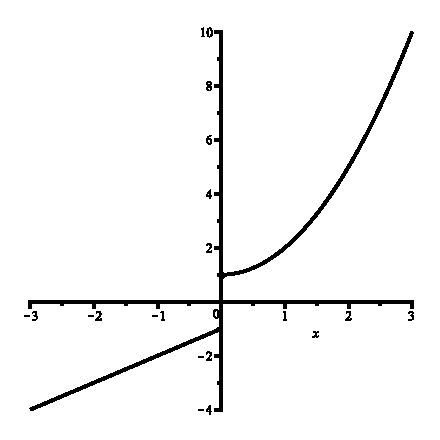
\includegraphics{fig-sec63-exer18.eps}
\end{center}
\end{figure}

\newpar
The function $f$ is an injection but is not a surjection.  To prove that it is an injection, let $a, b \in \R$ and assume that $f(a) = f(b)$.  There are four cases.
\begin{itemize}
\item $a \geq 0$ and $b < 0$.  This is not possible since in this case, $f(a) \geq 0$ and 
$f(b) < -1$.
\item $a < 0$ and $b \geq 0$.  This is not possible since in this case, $f(a) < -1$ and 
$f(b) \geq 0$.
\item $a \geq 0$ and $b \geq 0$.  In this case, $a^2 + 1 = b^2 + 1$ and hence, $a^2 = b^2$.  Since both $a$ and $b$ are nonnegative, $a = b$.
\item $a < 0$ and $b < 0$.  In this case, $a - 1 = b - 1$ and hence, $a = b$.
\end{itemize}
Therefore, $f$ is an injection.  To prove that $f$ is not a surjection, we note that if 
$x \geq 0$, then $f(x) \geq 0$ and if $x < 0$, then $f(x) < -1$.  Therefore, for all 
$x \in \R$, $f(x) \ne -0.5$.

\newpage
\item Following is a graph of the function $g$.
\begin{figure}[h]
\begin{center}
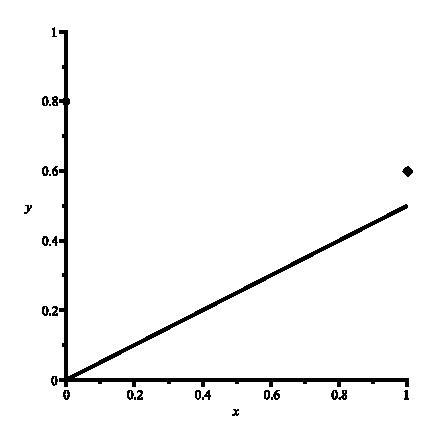
\includegraphics{fig-sec63-exer18b.eps}
\end{center}
\end{figure}
\newpar
The function $g$ is an injection but is not a surjection.  To prove that it is an injection, we first note that for each $x$ with $0 < x < 1$, $0 < g(x) < 0.5$.  In addition, $g(0) = 0.8$ and $g(1) = 0.6$.  From this we conclude that
\begin{itemize}
  \item For each $x$ with $0 < x \leq 1$, $g(0) \ne g(x)$.
  \item For each $x$ with $0 \leq x < 1$, $g(1) \ne g(x)$.
\end{itemize}
Now let $a, b \in [0, 1]$ and assume that $g(a) = g(b)$.  From the observations above, we can conclude that $0 < a < 1$ and $0 < b < 1$.  Hence, $g(a) = 0.5a$ and $g(b) = 0.5b$. Therefore, $g(a) = g(b)$ implies that $0.5a = 0.5b$ and hence, $a = b$.  This proves that $g$ is an injection.  To prove that $g$ is not a surjection, we note that $g(0) = 0.8$, $g(1) = 0.6$ and for each $x$ with $0 < x < a$, $0 < g(x) < 0.5$.  Therefore, for all $x$ in $[0, 1]$, $g(x) \ne =0.9$ and this proves that $g$ is not a surjection.


\item The function $h$ is not an injection since $h(0) = 0$ and $h(2) = 0$.  Since the codomain of $h$ is the set $\{0, 1\}$, and $h(0) = 0$ and $h(1) = 1$, we see that $h$ is a surjection.
\end{enumerate}

\end{document}
